\documentclass[a4paper,10pt]{report}
\usepackage[utf8]{inputenc}
\usepackage{graphicx}
\usepackage{float}
\usepackage{tikz}
\usepackage{pgfplots}

%\usepackage{geometry}
% \geometry{
% a4paper,
% total={170mm,257mm},
% left=20mm,
% top=20mm,
% }

\usepackage[margin=1in]{geometry}

% Title Page
\title{Results and Analysis}
\author{Kapil Thakkar and Reshma Kumari}


\begin{document}
\maketitle

% \chapter{Results and Analysis}



\begin{figure}[H]
\centering
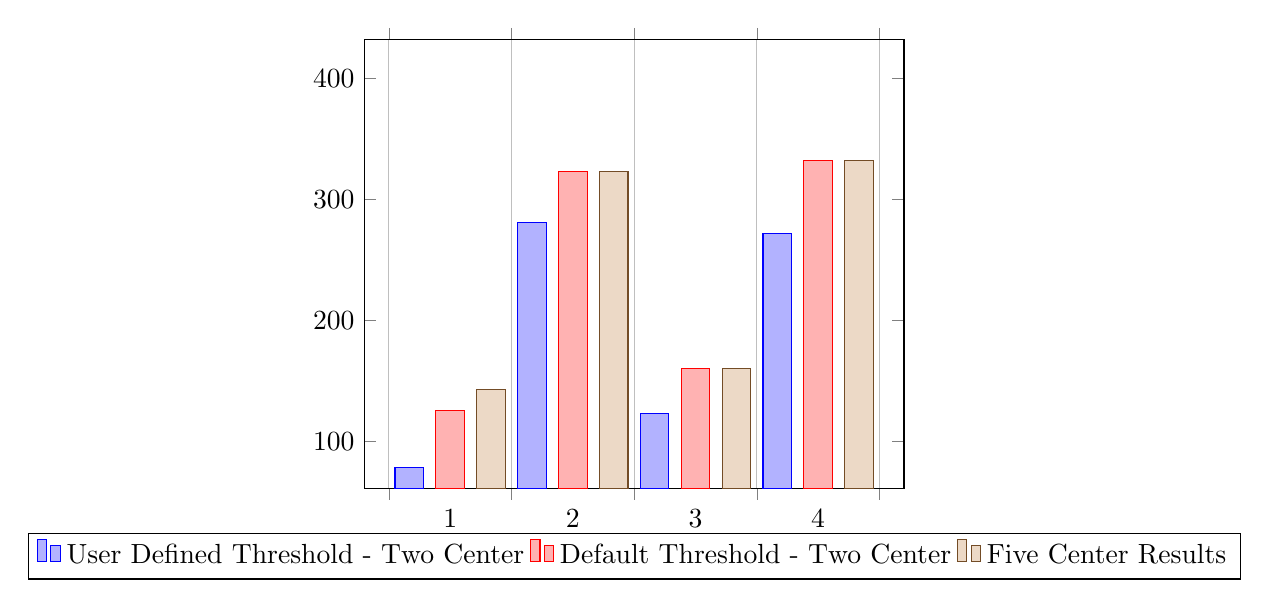
\begin{tikzpicture}
\begin{axis}[
	x tick label style={
		/pgf/number format/1000 sep=},
	enlargelimits=0.05,
	legend style={at={(0.5,-0.1)},
	anchor=north,legend columns=-1},
	ybar interval=0.7,
]
\addplot 
	coordinates {(1,78) (2,281)
		 (3,123) (4,272) (5,415)};
\addplot 
	coordinates {(1,125) (2,323)
		 (3,160) (4,332) (5,415)};
\addplot 
	coordinates {(1,143) (2,323)
		 (3,160) (4,332) (5,415)};
		
\legend{User Defined Threshold - Two Center, Default Threshold - Two Center, Five Center Results}
\end{axis}
\end{tikzpicture}
\caption{Anomaly Reported, (Retail vs Average Retail - 1, Retail vs Arrival - 2, Retail vs Wholesale - 3, Wholesale vs Arrival - 4)}
\label{fig:anomaliesReported}
\end{figure}



\begin{figure}[H]
\centering
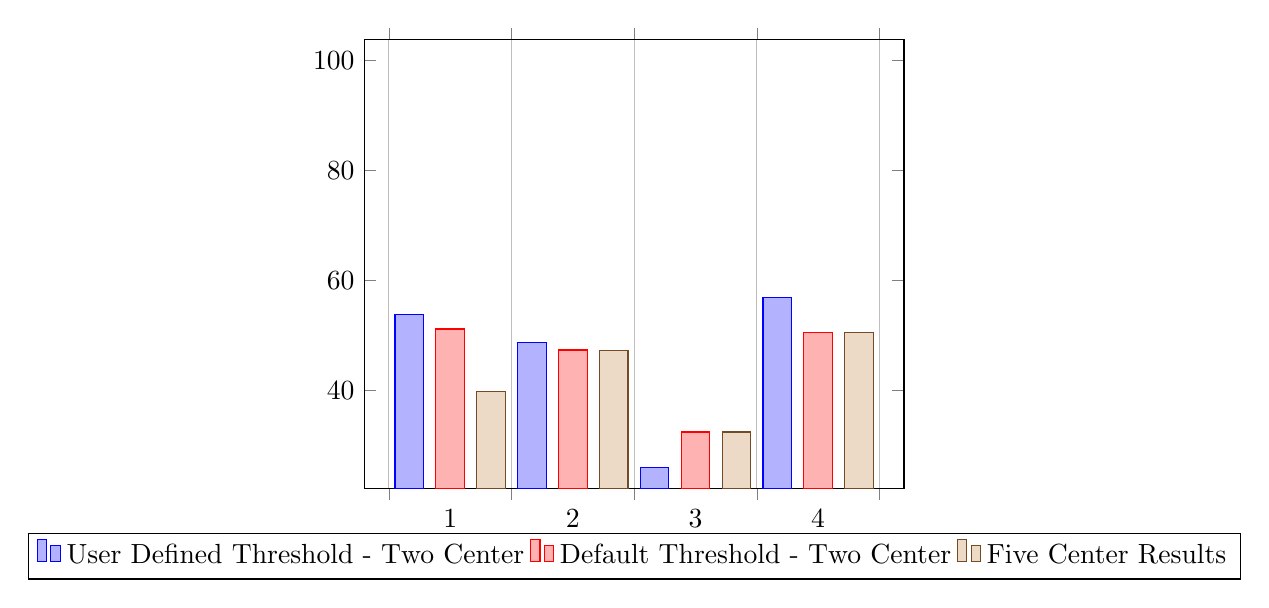
\begin{tikzpicture}
\begin{axis}[
	x tick label style={
		/pgf/number format/1000 sep=},
	enlargelimits=0.05,
	legend style={at={(0.5,-0.1)},
	anchor=north,legend columns=-1},
	ybar interval=0.7,
]
\addplot 
	coordinates {(1,53.85) (2,48.75)
		 (3,26.01) (4,56.99) (5,100)};
\addplot 
	coordinates {(1,51.2) (2,47.37)
		 (3,32.5) (4,50.6) (5,100)};
\addplot 
	coordinates {(1,39.86) (2,47.36)
		 (3,32.5) (4,50.6) (5,100)};
		
\legend{User Defined Threshold - Two Center, Default Threshold - Two Center, Five Center Results}
\end{axis}
\end{tikzpicture}
\caption{Precentage of Anomalies Matched, (Retail vs Average Retail - 1, Retail vs Arrival - 2, Retail vs Wholesale - 3, Wholesale vs Arrival - 4)}
\label{fig:percAnomaliesMatched}
\end{figure}

\end{document}          
